\begin{pa} \label{PA:2.2}
Consider the function $g(x) = 2^x$, which is graphed in Figure~\ref{F:2.2.PA1}.
\ba
	\item At each of $x = -2, -1, 0, 1, 2$, use a straightedge to sketch an accurate tangent line to $y = g(x)$.
	\item Use the provided grid to estimate the slope of the tangent line you drew at each point in (a).
	\item Use the limit definition of the derivative to estimate $g'(0)$ by using small values of $h$, and compare the result to your visual estimate for the slope of the tangent line to $y = g(x)$ at $x = 0$ in (b).
	\item Based on your work in (a), (b), and (c), sketch an accurate graph of $y = g'(x)$ on the axes adjacent to the graph of $y = g(x)$.
	\item Write at least one sentence that explains why it is reasonable to think that $g'(x) = cg(x)$, where $c$ is a constant.  In addition, calculate $\ln(2)$, and then discuss how this value, combined with your work above, reasonably suggests that $g'(x) = 2^x \ln(2)$.
\ea
\begin{figure}[h]
\begin{center}
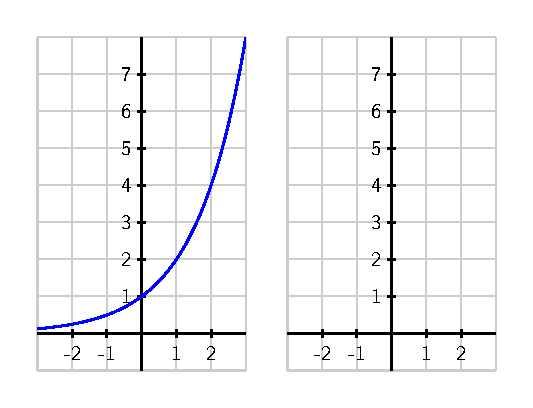
\includegraphics{figures/2_2_PA1a.eps}
\caption{At left, the graph of $y = g(x) = 2^x$. At right, axes for plotting $y = g'(x)$.} \label{F:2.2.PA1}
\end{center}
\end{figure}
\end{pa} \afterpa